\documentclass[11pt,letterpaper]{article}
\usepackage[margin=1in,bottom=1.1in]{geometry}
\usepackage{mathptmx}
\usepackage[T1]{fontenc}
\usepackage{fancyhdr,booktabs,enumitem,titlesec,tikz,caption}
\usetikzlibrary{positioning,arrows.meta}
\pagestyle{fancy}\fancyhf{}
\lhead{ARCTIC Research Allocation Proposal}\rhead{Parag Tamhankar}
\rfoot{\thepage}
\renewcommand{\headrulewidth}{0.4pt}
\titleformat{\section}{\normalfont\bfseries}{\Roman{section}.}{0.5em}{}
\titlespacing*{\section}{0pt}{9pt}{3pt}
\setlist{nosep,leftmargin=1.4em}
\setlength{\parskip}{5pt}\setlength{\parindent}{0pt}
\captionsetup{font=small,labelfont=bf,labelsep=colon,skip=3pt}
\raggedbottom\clubpenalty=0\widowpenalty=0\setlength{\textfloatsep}{8pt plus 2pt minus 2pt}
\begin{document}
\begin{center}
{\bfseries Specialized LLM Skills Across Fixed Quantitative Portfolio Optimization Strategies}
\end{center}

\textbf{Abstract}

Large language models (LLMs) can read financial news and rate stocks, but it is not known which portfolio strategies actually benefit from those ratings, or whether giving a model specialized instructions (``skills'') makes its ratings more useful. For my MS research project, supervised by Dr.\ Parag Tamhankar, I am running a controlled weekly study on live market data. Open-weight LLMs rate 100 to 300 S\&P 500 stocks each week, the ratings are turned into inputs for five fixed portfolio optimization strategies, and each strategy is compared with the same strategy run without any LLM input. I am requesting ARCTIC resources only for the LLM ratings, which run through ARCTIC's LiteLLM gateway on the existing Gemma 4 31B and MiniMax M2.7 models. The price forecaster, optimization, and statistical testing run on my own computer.

\section{Scientific Background}
Portfolio optimization turns expected stock returns and a measure of risk into portfolio weights. The standard tools, such as mean-variance optimization, are very sensitive to errors in the expected returns, so most practical systems combine a neutral market estimate with ``views'' about individual stocks using the Black-Litterman model. Recent studies feed LLM forecasts into these views and report that the best-performing LLMs beat standard baselines on risk-adjusted returns. Most of that work has three gaps. It tests one optimizer at a time, so it cannot say which strategies benefit from LLM views. It tests on historical data, where the LLM may already have read news about the period it is predicting, which inflates results. And it rarely checks whether better results come from the content of the prompt or simply from a longer prompt.

This project is built around those gaps. It holds the data, the risk estimate, the way views are built, and the trading rules fixed, and it changes only two things: which LLM ratings are used, and which optimization strategy uses them. It runs live, week by week, so the models cannot have seen the outcomes. It compares four specialized skills prompts with a bare prompt and a same-length placebo. My aims are:
\begin{enumerate}
\item[\textbf{1:}] Measure how often LLM ratings alone rank stocks better than a quantitative baseline.
\item[\textbf{2:}] Measure how LLM views change five optimization strategies, and which ones they help or hurt most.
\item[\textbf{3:}] Determine whether specialized skills, the choice of model, and market conditions change the effect.
\end{enumerate}
\textbf{Hypothesis:} LLM views improve on the quantitative baseline for some strategies but not others, and the size of the improvement depends on the strategy and on whether the model is given specialized skills.

\textbf{Expected outcomes:} The results will form my MS project and a conference paper submission. All code, prompts, and weekly data are versioned, so every result traces back to its exact inputs and other researchers can repeat the whole study from the same inputs.

\section{Computational Methods}
\textbf{A. Weekly pipeline:} Every Friday after the market closes, the pipeline freezes that week's public data (daily prices, news headlines, and earnings dates). Over the weekend it produces new portfolio weights, which are locked before the Monday open. Figure 1 shows the steps. The same pipeline, data, and trading rules are used for every model and strategy, so any difference in results comes from the LLM ratings or the strategy.

\begin{figure}[!t]\centering
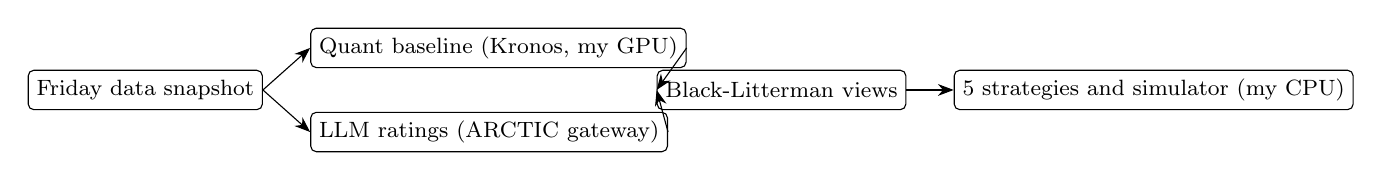
\begin{tikzpicture}[node distance=0.5cm, every node/.style={draw, rounded corners=2pt, align=center, font=\footnotesize, minimum height=0.5cm, inner sep=3pt}, >={Stealth[length=2mm]}]
\node (d) {Friday data snapshot};
\node (k) [above right=0.02cm and 0.6cm of d] {Quant baseline (Kronos, my GPU)};
\node (l) [below right=0.02cm and 0.6cm of d] {LLM ratings (ARCTIC gateway)};
\node (b) [right=5.0cm of d] {Black-Litterman views};
\node (s) [right=0.6cm of b] {5 strategies and simulator (my CPU)};
\draw[->] (d.east)--(k.west); \draw[->] (d.east)--(l.west); \draw[->] (k.east)--(b.west); \draw[->] (l.east)--(b.west); \draw[->] (b)--(s);
\end{tikzpicture}
\caption{The weekly pipeline. The baseline and LLM ratings are computed separately, then combined into views.}
\end{figure}

\textbf{B. Quant baseline:} Each stock is ranked on price momentum and on a five-day return forecast from Kronos, a pretrained forecasting model for price data (102M parameters). Kronos samples 20 possible price paths per stock, and the spread of those paths sets how much weight the baseline view gets.

\textbf{C. LLM ratings:} Each open-weight model rates each stock separately. The model sees the stock's ticker, company name, sector, and that week's news, and it returns a short JSON answer: a low, most likely, and high score on a $-5$ to $5$ scale, plus a one-sentence reason. A narrow range (for example 3 to 5) signals more confidence than a wide one (1 to 5), and the pipeline gives confident views more weight. Every stock is rated under six prompt types: a bare prompt, four specialized skills prompts of similar length, and a placebo prompt of the same length with no investing content. All calls use temperature 0 and a fixed seed. Because the gateway batches requests from many users, repeated answers can still differ slightly, so the pilot rates a fixed set of stocks twice to measure how often ratings agree, and a small fixed set of check prompts runs at the start of each weekend to catch model changes. Each request's token counts, including MiniMax's reasoning tokens, and the gateway's model and deployment IDs are logged, so my usage can be checked against the allocation at any time.

\textbf{D. Strategies and evaluation:} The ratings are combined with the baseline through Black-Litterman and passed to five fixed strategies: mean-variance, mean-CVaR (which balances return against the average loss in the worst 5\% of outcomes, using 10,000 simulated scenarios), robust mean-variance, resampled mean-variance, and a top-20 portfolio. Each strategy also runs a control portfolio every week that uses the baseline alone, and two more controls (hierarchical risk parity and equal weight) use no forecasts at all. A trade simulator applies the same rules to every portfolio: weekly rebalancing, daily stop-loss and take-profit checks, and a 0.1\% cost per trade. The statistical tests use only the saved ratings, weights, and returns, so they rerun no models or optimizers and take minutes on my own computer.

\section{Software}
The pipeline uses Python 3.11 with pandas, NumPy, SciPy, scikit-learn, statsmodels, and cvxpy, with PyTorch for Kronos. Each weekend the pipeline runs on my own computer, which sends the LLM requests to ARCTIC's OpenAI-compatible LiteLLM endpoint over the GSU VPN, so both models use the same code and settings. Kronos, the optimization, and the simulator run locally. I request:
\begin{itemize}
\item \textbf{Existing models:} Gemma 4 31B and MiniMax M2.7, already on the gateway, so I am not requesting any new model deployments or changes to the gateway.
\item \textbf{Use pattern:} one stock per request, about 300 to 8,000 input tokens each, and about 300 output tokens for Gemma 4 31B or up to about 2,000 for MiniMax M2.7, whose reasoning counts as output. Requests are sent in a 48-hour weekend window with both models in parallel (up to four at a time per model) and no images, tools, or web access. At full scale that is about 4,200 requests per weekend window, roughly 1 to 34 million input tokens and about 4.8 million output tokens in total.
\item \textbf{Duration:} 12 months from approval, with heavy use only in about 24 weekend windows. I plan to start the pilot as soon as access is available, ideally in early December 2026, and the live run continues through the spring 2027 semester.
\end{itemize}
If the gateway is down during a weekend run, that model's week is left out of its statistics. Two small commercial API models (Claude Haiku 5.5 and GPT-6 Luna) are also rated for comparison on their providers' servers, using no ARCTIC compute. All inputs are public market data and published news, with no personal or regulated data. ARCTIC's hosted models are approved for unregulated university data, models banned by GSU's tool registry (such as Qwen) are not used, and papers will disclose AI use.

\section{Justifying Allocation Amounts}
The LLM ratings are the one part of the project that needs ARCTIC: Gemma 4 31B and MiniMax M2.7 are far too large for my own GPU, which has 6 GB of memory, and ARCTIC already hosts both. The rest of the pipeline fits on my own computer.

The estimate is for the largest planned configuration: 300 stocks, two open-weight models, and about 24 weeks of pilot and live runs. I plan six prompt types and size the request for seven, so a fifth skills file can be added. Each week that is 300 $\times$ 7 $\times$ 2 = 4,200 LLM requests. I estimate about 40 GPU-seconds per Gemma request and about 90 per MiniMax request in V100-equivalent time, based on each model's size and memory bandwidth; MiniMax costs more because it writes up to about 2,000 output tokens. Because the way gateway use is counted is still being set up, Table 1 also lists the weekly token totals.

\begin{table}[!t]\centering\setlength{\tabcolsep}{5pt}
\caption{Estimated ARCTIC usage and request for the two options.}
\small
\begin{tabular}{lrrrrr}
\toprule
Option & Requests/week & Tokens/week (in; out) & Weeks & Estimated use & Request \\
\midrule
300 stocks (preferred) & 4,200 & 1.3 to 34M; 4.8M & 24 & 1,820 GPU-hours & 2,730 GPU-hours \\
100 stocks (smaller) & 1,400 & 0.4 to 11M; 1.6M & 24 & 607 GPU-hours & 910 GPU-hours \\
\bottomrule
\end{tabular}
\end{table}

Each model handles 2,100 requests a week at 300 stocks. Over 24 weeks that is about 560 GPU-hours for Gemma and 1,260 for MiniMax, or 1,820 in total. The request adds about 50\% for failed calls, retries, test and check calls, and a longer live run. I need no CPU hours, because the optimization, simulation, and statistical tests run locally, and no storage beyond the default project space, because rating records are small (about 1 KB each) and are saved on my own computer, where the rest of the analysis also runs.

\textbf{Smaller option:} I prefer 300 stocks, but the number of stocks is a setting in my pipeline, and the study still answers its main question with 100. If ARCTIC can approve only a smaller request, I will run it with 100 stocks instead, as the second row of Table 1 shows.

\end{document}
